% !TEX root = omar-thesis.tex
\chapter{Introduction}\label{chap:intro}
% \vspace{-14px}
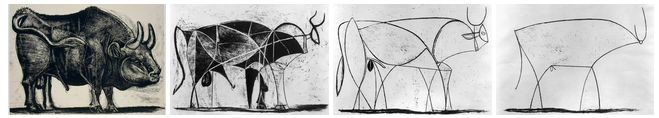
\includegraphics[width=\textwidth]{Picasso-Bull-Progression-cropped.png}
\begin{flushright}
\emph{Bull} (plates 3, 6, 9 and 11)\\
Pablo Picasso (1881-1973)\end{flushright}
% http://www.artyfactory.com/art_appreciation/animals_in_art/pablo_picasso.htm
%\vspace{-5px}
% \begin{quote}\textit{The recent development of programming languages suggests that the simul\-taneous achievement of simplicity 
% and generality in language design is a serious unsolved 
% problem.}\begin{flushright}--- John Reynolds (1970) \cite{Reynolds70}\end{flushright}
% \end{quote}
%\begin{quote}
%\textit{Try to imagine that you are a tree. How do you want to look out here?}
%\textit{You want your tree to have some character.}
%\begin{flushright} --- Bob Ross, \emph{The Joy of Painting}\end{flushright}
%\end{quote}

% \vspace{-7px}
\section{Motivation}\label{sec:intro-motivation}
% \vspace{-6px}
%Programming languages come in many sizes. The smallest languages -- for example, the various ``lambda calculi'' -- isolate language primitives of interest for the benefit of students, researchers and language designers interested in studying their mathematical properties. These studies inform the design of ``full-scale'' programming 
%\footnote{Throughout this work, words and phrases that should be read as having an intuitive or informal meaning, rather than a strict mathematical meaning, will be introduced with quotation marks.} 
% languages, which combine several such primitives, or generalizations thereof. Full-scale languages are interesting objects of formal study in their own right. They also serve as useful tools for software developers, allowing them to construct, reason about and modularly organize large software systems.
% A single mathematical structure can often take on many syntactic forms. 
% Formal mathematical structures often come equipped with
% Experienced mathematicians and programmers define formal structures \emph{compositionally}, drawing from libraries by instantiating more abstract structures. This ultimately increases productivity, because clients of these abstract structures do not need to expend effort to establish the associated definitions and proofs anew, for each specialized structure of interest. %Instead, they need only instantiate the definitions and proofs established by a library provider in a more abstract setting.

Experienced mathematicians and programmers define formal structures \emph{compositionally}, drawing from libraries of ``general-purpose'' abstractions. The problem that motivates this work is that the resulting terms are sometimes syntactically unwieldy, and, therefore, cognitively costly. % This can neutralize the cognitive benefits of abstraction and composition. We go, therefore, in search of a mechanism of syntactic control that maintains strong compositional reasoning principles. %This can lower productivity, readability and other quality attributes of interest.  %This saves time, one does not need to establish associated definitions and proofs anew, for each specialized structure of interest.

Consider, for example, natural numbers. It is straightforward to define the natural numbers, $n$, with an inductive structure:
\[ n ::= \textbf{z} ~\vert~ \textbf{s}(n)\]
By defining natural numbers inductively, we immediately inherit a \emph{structural induction principle} -- we can establish that some property $P$ holds over the natural numbers if we establish $P(\textbf{z})$ and $P(\textbf{s}(n))$ assuming $P(n)$. The problem, of course, is that drawing particular natural numbers by repeatedly applying $\textbf{s}$ very quickly becomes syntactically unwieldy (in fact, the syntactic cost of the drawing grows linearly with $n$.)\footnote{We use the word ``drawing'' throughout this document to emphasize that syntactic cost is a property of the visual representation of a structure, rather than a semantic property.}

Similarly, it is easy to define lists of natural numbers with an inductive structure:
\[ \vec{n} ::= \textbf{nil} ~\vert~ \textbf{cons}(n, \vec{n}) \]
The problem once again is that drawings of particular lists quickly become unwieldy, and fail to resemble ``naturally occurring'' drawings of lists of numbers.

Consider a third more sophisticated example (which will be of particular relevance later in this work): when defining a programming language or logic, one often needs various sorts of tree structures equipped with metaoperations\footnote{...so named to distinguish them from the ``object level'' operations of the language being defined.} related to variable binding, e.g. substitution. Repeatedly defining these structures ``from scratch'' is quite tedious, so language designers have instead developed  a more general structure: the \emph{abstract binding tree (ABT)} \cite{Aczel78,pfpl,gabbay2002new}. Briefly, an ABT is an ordered tree structure, classified into one of several \emph{sorts}, where each node is either a \emph{variable}, $x$, or an \emph{operation} of the following form:
%\footnote{Some prior exposure to (single-sorted) ASTs is assumed here. See Sec. \ref{sec:preliminaries} for other preliminaries.} 
\begin{equation*}
\abop{op}{\vec{x}_1.\mathit{a}_1; \ldots; \vec{x}_n.\mathit{a}_n}
\end{equation*} 
where $\texttt{op}$ identifies an \emph{operator} and each of the $n \geq 0$ \emph{arguments} $\vec{x}_i.\mathit{a}_i$ binds the (possibly empty) sequence of variables $\vec{x}_i$ within the subtree $a_i$. The left side of the syntax chart in Figure \ref{fig:simple-example} summarizes the relevant operational forms for a sort called $\mathsf{CalcExp}$. ABTs of this sort are the expressions of a small arithmetic programming language,  $\simplelang$. By using  ABTs as infrastructure in the definition of $\simplelang$, we need not manually define the ``boilerplate'' metaoperations, like substitution, and reasoning principles, like structural induction, that are necessary to define $\simplelang$'s semantics and to prove it correct. {Harper gives a detailed account of ABTs, and many other examples of their use, in his book \cite{pfpl}.} 

 %and reasoning principles, e.g. {structural induction}, so we need not define this  machinery manually. 
% -- the arities of the operators can be read off from these forms ($\anumintro{n}$ is a number-indexed family of nullary operators.) 

\begin{figure}
\hspace{-5px}$\begin{array}{lrlllll}
\textbf{Sort} & & & \textbf{Operational Form} & \textbf{Stylized Form} & \textbf{Textual Form} & \textbf{Description}\\
\mathsf{CalcExp} & e & ::= & x & x & x & \text{variable}\\
&&& \aletplain{e}{x}{e} & \letplain{x}{e}{e} & \letplain{x}{e}{e} & \text{binding}\\
&&& \anumintro{n} & \numintro{n} & \numintro{n} & \text{numbers}\\
&&& \aplus{e}{e} & e + e & e\texttt{ + }e & \text{addition} \\
% &&& \aminus{e}{e} & e - e & e\texttt{ - }e & \text{subtraction}\\
&&& \amult{e}{e} & e \times e & e\texttt{ * }e & \text{multiplication}\\
&&& \adiv{e}{e} & \frac{e}{e} & e\texttt{ / }e & \text{division}\\
&&& \apow{e}{e} & {e}^{e} & e\verb|^|e & \text{exponentiation}\\
\end{array}$
\caption[Syntax of $\simplelang$]{Syntax of $\simplelang$. Metavariable $n$ ranges over natural numbers and $\numintro{n}$ abbreviates the numeral forms (one for each natural number $n$, drawn in \texttt{typewriter} font.) A formal definition of the stylized and textual syntax of $\simplelang$ would require 1) defining these numeral forms explicitly; 2) defining a parenthetical form; 3) defining the precedence and associativity of each infix operator; and 4) defining whitespace conventions.}
\label{fig:simple-example}
% \vspace{-5px}
\end{figure}

% \subsection{Syntax Matters}
The problem with this approach is, again, that drawing a non-trivial $\simplelang$ expression in operational form is syntactically costly. For example, we will consider the following drawing in our discussion below:
\begin{subequations}\label{drawings:simple}\begin{equation}\label{simple-example-op-form}
\adiv{\anumintro{\textbf{s}(\textbf{z})}}{
	\apow{\anumintro{\textbf{s}(\textbf{s}(\textbf{z}))}}{\adiv{\anumintro{\textbf{s}(\textbf{z})}}{\anumintro{\textbf{s}(\textbf{s}(\textbf{z}))}}}
}\end{equation}
% This is an example of a common problem: instantiating a general-purpose abstraction, here for defining ABTs, can be  structurally economical but  \emph{syntactically costly} (or \emph{cognitively costly} in some other sense, as we will discuss in Section \ref{sec:syntactic-properties}.) Mathematics is ultimately a human activity, so these costs are worthy of consideration.

\subsection{Informal Mathematical Practice}
Within a document intended only for human consumption, it is easy to informally outline less costly alternative syntactic forms. 

For example, mathematicians generally use the Western Arabic numeral forms when drawing particular natural numbers, e.g. $2$ is taken as a syntactic alternative to $\textbf{s}(\textbf{s}(\textbf{z}))$. 

Similarly, mathematicians might informally define alternative list forms, e.g. $[0, 1, 2]$ as a syntactic alternative to: 
\[\textbf{cons}(\textbf{z}, \textbf{cons}(\textbf{s}(\textbf{z}), \textbf{cons}(\textbf{s}(\textbf{s}(\textbf{z})), \textbf{nil})))\]

The middle columns of the syntax chart in Figure \ref{fig:simple-example} suggest two alternative forms for every ABT of sort $\mathsf{CalcExp}$. We can draw the ABT from Drawing (\ref{simple-example-op-form}) in an alternative \emph{stylized form}:
% div(num[1]; pow(num[2]; div(num[1]; num[2]))
% \begin{subequations}
% \begin{equation}\label{simple-example-op-form}
% \adiv{\anumintro{1}}{
% 	\apow{\anumintro{2}}{\anumintro{3}}
% }\end{equation}
\begin{equation}\label{simple-example-sty-form}
\frac{\numintro{1}}{{\numintro{2}^{\frac{\numintro{1}}{\numintro{2}}}}}
\end{equation}
or in an alternative \emph{textual form}:
\begin{equation}\label{simple-example-txt-form}
\texttt{1 / 2\textasciicircum(1/2)}
\end{equation}
\end{subequations}

Mathematicians also sometimes supplement alternative primitive forms like these with various \emph{derived forms}, which  identify ABTs indirectly according to stated context-independent \emph{desugaring rules}. For example, the following desugaring rule defines a derived stylized form for square root calculations:
% \begin{subequations}
% \begin{subequations}[intermezzo]
\begin{equation}\label{rule:simplelang-sqrt}
\sqrt{e} \rightarrowtriangle e^{\frac{\numintro{1}}{\numintro{2}}}
\end{equation}
% \end{subequations}
The reader can desugar a drawing of an ABT by recursively applying desugaring rules wherever a syntactic match occurs. A desugared drawing consists only of the {primitive forms} from Figure \ref{fig:simple-example}. 
For example, the following drawing desugars to Drawing (\ref{simple-example-sty-form}), which in turn corresponds to Drawing (\ref{simple-example-op-form}) as discussed above:
\begin{equation*}\tag{\ref*{drawings:simple}d}
\frac{\numintro{1}}{\sqrt{\numintro{2}}}
\end{equation*}
%No new operators are introduced.

% Syntactically, however, this practice has its limits. 

% Mathematicians often invent specialized syntactic forms in order to visually represent the formal structures that they define. 
% % For example, Figure \ref{fig:simple-example} defines three different ways to draw any abstract syntax tree (AST) of sort  $\mathsf{CalcExp}$. ASTs of this sort are the expressions of a small arithmetic programming language, $\simplelang$.\footnote{Some familiarity with abstract syntax trees is preliminary to this work. See Sec. \ref{sec:preliminaries} for citations and a more thorough discussion of preliminaries.}
% % Mathematicians, like painters, exercise creative license when they draw the structures that arise in their work. 
% % Mathematicians, like painters, exercise creativity when they draw the structures that arise in their work. 
% % Mathematicians often define structurally redundant syntactic forms. 
% %, i.e. forms that are syntactically distinct but that identify the same formal structure. 
% % When defining the syntax of a programming language, language designers often define structurally redundant syntactic forms. 
% % Mathematicians, like painters, draws these trees in a variety of styles.  
% % There are many ways to draw trees of this sort. 
% % There are many ways to draw a tree. 
% % Most formal structures are defined as modes of use of more primitive formal structures. For example, the expressions of a variety of programming languages are all defined as particular sorts of \emph{abstract syntax trees}.  
% For example, the three drawings below all identify the same tree structure  of sort $\mathsf{CalcExp}$, differing according to the syntax chart in Figure \ref{fig:simple-example} only in that the first drawing is in a general \emph{operational form}, whereas the second drawing is in a specialized \emph{stylized form} and the third is in a specialized \emph{textual form}:
% %
% % differing only in that Drawing (\ref*{simple-example-op-form}) is in \emph{operational form}, Drawing (\ref*{simple-example-sty-form}) is in \emph{stylized form} and Drawing (\ref*{simple-example-txt-form}) is in \emph{textual form}:
% \begin{subequations}
% \begin{equation}\label{simple-example-op-form}
% \adiv{\anumintro{1}}{
% 	\apow{\anumintro{2}}{\anumintro{3}}
% }\end{equation}
% \begin{equation}\label{simple-example-sty-form}
% \frac{\numintro{1}}{{\numintro{2}^{\numintro{3}}}}
% \end{equation}
% \begin{equation}\label{simple-example-txt-form}
% \texttt{1 / 2\textasciicircum3}
% \end{equation}
% \end{subequations}
% \noindent
% Trees of this sort are the expressions of $\simplelang$, a simple arithmetic programming language. 

% These drawings identify the same AST, meaning that they are all drawn from the same row of the syntax chart at every level. In other words, these drawings are structurally indistinct. 

% In particular, let us consider a simple programming language, $\simplelang$, for performing arithmetic calculations with numbers. The expressions of $\simplelang$ are \emph{abstract syntax trees (ASTs)} of a sort defined by the syntax chart in Figure \ref{fig:simple-example}.\footnote{Familiarity with abstract syntax trees is preliminary to this work (see Sec. \ref{sec:preliminaries} for other preliminaries.)}  For example, the following expression is drawn in stylized form:
% The same expression is drawn in textual form as follows:
% \noindent
% and in operational form as follows:

When defining the semantics of a language like $\simplelang$, it is customary to adopt an \emph{identification convention} whereby drawings that identify the same underlying ABT structure, like Drawings (\ref{drawings:simple}), are considered interchangeable. %only if they are drawn from different rows of the syntax chart in Figure \ref{fig:simple-example}. 
For example, consider the semantic  judgement $\isvalU{e}$, which establishes certain  $\simplelang$ expressions as \emph{values} (as distinct from expressions that can be arithmetically simplified or that are erroneous.) The following inference rule establishes that every number expression is a value:\footnote{Some familiarity with inductively defined judgements and inference rules like these is preliminary to this work. See Sec. \ref{sec:preliminaries} for citations and further discussion of necessary preliminaries.}
\begin{equation}\label{rule:num-val}
\inferrule{ }{
	\isvalU{\anumintro{n}}
}
\end{equation}
Although this rule is drawn using the operational form for number expressions, we can apply it to derive that $\isvalU{\numintro{2}}$, because $\numintro{2}$ and $\anumintro{2}$  identify the same ABT.

% In summary, it is both the case that ``syntax doesn't matter'' (semantically) and that syntax matters (cognitively). %i.e.  because mathematics is a human activity that alternative and derived forms matter (cognitively).%Syntax matters because mathematics and programming are human activities. 


% \subsection{Syntax Doesn't Matter  (Semantically)}
% It is worth emphasizing here that these common syntactic practices are not motivated by semantic considerations. Indeed, 



% \subsection{Syntax Matters (Cognitively)}
% %Our semantics would be no weaker if we had defined only, for example, the operational forms. 
% %The answer, of course, is that from the perspective of a human programmer, syntax \emph{does} matter. 
% % If different drawings of a $\simplelang$ expression are not semantically distinguishable, why did we bother to define alternative syntactic forms at all?
% Syntactic sugar matters because mathematics and programming are human activities. Different visual representations of a formal structure can and must be distinguished by the \emph{cognitive costs} that human programmers incur as they produce or examine them.\footnote{In fact, we should be interested in sensory modalities other than vision, if only because many humans lack sufficient eyesight. Alas, this topic is beyond the scope of our present work.}% Drawings of formal structures serve as \emph{user interfaces} to the underlying structures themselves.

% For example, a human programmer might distinguish drawings of $\simplelang$ expressions in stylized or textual form, like Drawings (\ref{simple-example-sty-form}) through (\ref{simple-example-derived-form}) above, as less ``crowded'' and more ``familiar'' than those in operational form, because they follow the usual arithmetic conventions or close approximations thereof. This might help the human  programmer extract meaning from such drawings more quickly. Similarly, drawings in textual form involve only text, which can lower the costs involved in their production. Of course, drawings in operational form can bring cognitive benefits as well -- dispensing with various syntactic complexities (e.g. related to  precedence and associativity) can simplify metatheoretic reasoning and implementation efforts. 

% We will cover more rigorous operationalizations of the necessarily broad notion of cognitive cost in Section \ref{sec:syntactic-properties}. %Mistakes may also be less frequent when producing drawings in stylized or textual form (for $\simplelang$ expressions, perhaps only because operational forms use more parentheses). 

% \subsection{Derived Forms}
% %The forms defined by the syntax chart in Figure \ref{fig:simple-example} suffice to allow programmers to draw any $\simplelang$ expression. However, 
% In seeking to lower cognitive costs, syntax designers  often  include additional \emph{derived forms}  in a syntax definition. Unlike the \emph{primitive forms}  defined in Figure \ref{fig:simple-example}, which identify trees directly, derived forms identify trees indirectly, through a context-independent {desugaring} rule.   
% %We can define a desugaring transformation by stating a rewrite rule. 
% For example, the following desugaring rule defines a derived stylized form for calculating the square root of a $\simplelang$ expression:
% % \begin{subequations}
% \begin{equation}\label{rule:simplelang-sqrt}
% \sqrt{e} \rightarrowtriangle e^{\frac{\numintro{1}}{\numintro{2}}}
% \end{equation}
% % Similarly, the following rewrite rule, if included in the definition of the textual syntax of expressions, defines a derived form for negating a $\simplelang$ expression:\footnote{Notice that the right-hand side of this rule is in operational form, rather than textual. For $\footnotesimplelang$, it is not necessary to prevent textual and operational forms from being interspersed within a single drawing -- no ambiguities can arise. For richer syntax definitions, this may no longer be the case. The desugaring process must then be modified to first convert the pattern on the righthand side of a desugaring rule like Rule (\ref{rule:simplelang-negate}) to the desired form variant before it is applied.}
% % \begin{equation}\label{rule:simplelang-negate}
% % \texttt{-}e \rightarrowtriangle \amult{e}{\anumintro{-1}}
% % \end{equation}
% % \end{subequations}
% % \noindent 
% Desugaring a drawing of a tree involves first recursively desugaring the drawings of its subtrees. If the drawing is in primitive form, desugaring is complete.  If the drawing is in derived form, we apply the corresponding desugaring rule (here, we  have only one choice.) The desugared drawing will identify a tree immediately, i.e. it will consist only of primitive forms. No new trees are introduced, so the semantics is unchanged. %Derived forms affect only cognitive cost.
%Similarly, we might define a derived form for taking an arbitrary root of an expression as follows:
% \begin{align*}
% \sqrt[e']{e} & \rightarrowtriangle e^{\frac{\numintro{1}}{e'}}
% \end{align*}

\subsection{Derived Forms in General-Purpose Languages}
We would need to define only a few more derived arithmetic forms to satisfyingly capture the  idioms that arise in the limited domains where a simple language of arithmetic operations like $\simplelang$ might be useful. %Consequently, there is little opportunity to go beyond simple derived forms like these. 
However, programming languages in common use today are substantially more semantically expressive. Indeed, many mathematical structures, including natural numbers, lists and ABTs, can be adequately expressed within contemporary ``general-purpose'' programming languages. %Mathematics has become supplanted by particular formal system. 
Consequently, the problems of syntactic cost just discussed at the level of the ambient mathematics also arise ``one level down'', i.e. when writing programs. For example, we want syntactic sugar not only for mathematical natural numbers, lists and $\simplelang$ expressions, but also for \emph{encodings} of these structures within a general-purpose programming language.% .) %https://github.com/jonsterling/sml-abt or https://github.com/RedPRL/sml-typed-abts.) 

We can continue to rely on the informal notational conventions described above only as long as programs are drawn solely for human consumption. These conventions break down when we need drawings of programs to themselves exist as formal structures suitable for consumption by other programs, i.e. \emph{parsers}, which check whether drawings are well-formed relative to a \emph{syntax definition} and produce structures suitable for consumption by yet other programs, e.g. compilers. %This, of course, is the regime of contemporary computer programming.

% The problem is that nearly all contemporary languages are designed so that drawings of programs can be consumption both by humans and by another program -- a parser -- which checks whether drawings are well-formed and produces a structure suitable for consumption by various other useful programs, e.g. editors and compilers.


% Programmers address these problems by informally stating alternative and derived forms, as in handwritten or typeset mathematics, because a drawing of a program must be suitable for consumption both by humans and by % This limits the control that programmers have over syntactic cost.

% In contemporary practice, other programs -- parsers -- consume drawings of programs, which generate corresponding structures for execution by modern computer hardware. As such, we cannot rely on an informal approach that defers ultimately to the intuitions of a human reader. Instead, we must define the syntactic conventions that we wish to use with rigor. 

Constructing a formal syntax definition is not itself an unusually difficult task for an experienced programmer, and there are many \emph{syntax definition systems} that help with this task (Sec. \ref{sec:existing-approaches} will cover several examples.) The problem is that when designing the syntax of a general-purpose language, the language designer cannot hope to anticipate all library constructs for which derived forms might one day be useful. At best, the language designer can bundle certain libraries together into a ``standard library'', and privilege select constructs defined in this library with derived forms. 

% as these ``general-purpose'' languages have evolved, many other derived forms have become incorporated into their syntax definitions.\footnote{The same dynamic is apparent in the progression of ``pen and paper'' and typeset mathematics.}  
For example, the textual syntax of Standard ML (SML), a general-purpose language in the functional tradition, defines derived forms for constructing and pattern matching on lists \cite{mthm97-for-dart,harper1997programming}. In SML, the derived expression form \lstinline{[x, y, z]} desugars to an expression equivalent to:
\begin{lstlisting}[numbers=none]
Cons(x, Cons(y, Cons(z, Nil)))
\end{lstlisting}
assuming \li{Nil} and \li{Cons} stand for the list constructors exported by the SML Basis library (i.e. SML's ``standard library''.)\footnote{The desugaring actually uses unforgeable identifiers bound permanently to the list constructors, to ensure that the desugaring is context independent. We will return to the concept of context independence throughout this work.} Other languages similarly privilege select standard library constructs with derived forms:

\begin{itemize}
\item OCaml \cite{ocaml-manual} defines derived forms for strings (defined as arrays of characters.)
\item Haskell \cite{jones2003haskell} defines derived forms for encapsulated commands (and, more generally, values of any type equipped with monadic structure.)
\item Scala \cite{odersky2008programming} defines derived XML forms as well as string splicing forms, which capture the idioms of string concatenation.
\item F\# \cite{syme2012expert}, Scala \cite{shabalin2013quasiquotes} and various other languages define derived forms for encodings of the language's own terms (these are referred to as \emph{quasiquotation} forms.)
\item Python \cite{python} defines derived forms for mutable sets and dictionaries.
\item Perl \cite{perlre} defines derived regular expression forms.
\end{itemize}

These choices are, fundamentally, made according to \emph{ad hoc} design criteria -- there are no clear semantic criteria that fundamentally distinguish standard library constructs privileged with derived forms from those defined in third-party libraries. 
%Indeed, it is considered a virtue for a standard library can be separated from the language definition. 
Indeed, as the OCaml community has moved away from a single standard library in favor of competing bundles of third-party libraries (e.g. Batteries Included \cite{OCaml-batteries} and Core \cite{OCaml-core}), this approach has become starkly impractical.% This puts into question the practice of bundling a single standard library with  entirely.

\section{Existing Mechanisms of Syntactic Control}
A more parsimonious approach would be to eliminate derived forms  specific to standard library constructs from language definitions in favor of mechanisms that give more syntactic control to third-party library providers.

In this section, we will give a brief overview of existing such mechanisms and speak generally about the problems that they present to motivate our novel contributions in this area. We will return to give a detailed overview of these various existing mechanisms of syntactic control in Section \ref{sec:existing-approaches}. 

\subsection{Syntax Dialects}\label{sec:problems-with-dialects}
One approach that a library provider can take when seeking more syntactic control is to use a syntax definition system to construct a \emph{syntax dialect}, i.e. a new syntax definition that extends the original syntax definition with new derived forms. 
%library-specific (a.k.a. ``domain-specific'') 

For example, Ur/Web extends Ur's textual syntax with derived forms for SQL queries, XHTML elements and other constructs defined in a  web programming library \cite{conf/popl/Chlipala15,conf/pldi/Chlipala10}. Figure \ref{fig:urweb} demonstrates how XHTML expressions that contain strings can be drawn in Ur/Web. The desugaring of this derived form (not shown) is substantially more verbose and, for programmers familiar with the standardized syntax for XHTML \cite{xhtml}, substantially more obscure. % Such dialects are sometimes qualitatively taxonomized as amongst the ``domain-specific language'' for this reason \cite{fowler2010domain}. %Syntactic cost is often assessed qualitatively \cite{green1996usability}, though quantitative metrics can be defined. 
\begin{figure}[h]
\begin{lstlisting}[numbers=none]
val p = SURL<xml><p>Hello, {[EURLjoin " " [first, last]SURL]}!</p></xml>EURL
\end{lstlisting}
\caption{Derived XHTML forms in Ur/Web}
\label{fig:urweb}
\end{figure}                           

Syntax definition systems like Camlp4 \cite{ocaml-manual}, Copper \cite{conf/gpce/WykS07} and SugarJ/Sugar* \cite{erdweg2011sugarj,erdweg2013framework}, which we will discuss in Sec. \ref{sec:syntax-dialects}, have simplified the task of defining ``library-specific'' (a.k.a. ``domain-specific'') syntax dialects like Ur/Web, and have thereby contributed to their ongoing proliferation.
%The desugaring, not shown, is substantially more verbose and, for programmers who are familiar with XHTML forms, substantially more obscure than the drawing above. %We will consider other examples of data structures where syntactic cost becomes a legitimate concern for client programmers in Sec. \ref{sec:motivating-examples}. 
%after first reviewing simpler approaches that also help library providers control syntactic cost, albeit to a more limited extent, 
% Syntax definition systems 
% The most syntactically expressive of the mechanisms that we will detail in Section \ref{sec:existing-approaches} are 


%Full-scale languages are also interesting objects of mathematical study. Uniquely, however, they are also designed for use by humans. Consequently, their designers  typically define both an abstract syntax and a textual syntax. This textual syntax serves as the primary interface between human programmers and the language, so it is common to define various \emph{derived forms}, i.e. forms defined by a context-independent \emph{desugaring} to a set of \emph{base forms}. These serve to decrease the \emph{syntactic cost} or \emph{cognitive cost} of selected idioms. 
%In some cases, a derived form is designed to capture an idiom77Gu that involves only the primitive constructs of the language. 

%The hope amongst some language designers is that a limited number of derived forms like these will suffice to produce a ``general-purpose'' textual syntax, i.e. one that is accepted as suitable for use across a wide variety of application domains. Alas, a stable design that fully achieves this ideal has yet to emerge, as evidenced by the diverse array of \emph{syntax dialects} -- dialects that introduce only new derived forms -- that continue to proliferate around all major contemporary languages. 

%In fact, tools that aid in the construction of so-called  ``domain-specific'' language dialects (DSLs)\footnote{In some parts of the literature, such dialects are called ``external DSLs'', to distinguish them from  ``internal'' or ``embedded DSLs'', which are actually  library interfaces that only ``resemble'' distinct dialects \cite{fowler2010domain}.} seem only to be becoming more prominent over time. 

%\subsection{Why are there so many language dialects?}
%{This calls for an investigation}: why is it that programmers and researchers are still so often unable to satisfyingly express the constructs that they seek in libraries, as modes of use of the ``general-purpose'' primitives already available in major languages today, and instead see a need for new language dialects?

%Perhaps the most common sort of dialect is the \emph{syntax dialect} -- a dialect that introduces only new derived syntactic forms, motivated by a desire to decrease the {syntactic cost} of working with one or more library constructs of interest. 
%Put another way, syntax dialects can be specified by a context-independent expansion to the existing language that they are based on. 
%For example, Ur/Web is a syntax dialect of Ur (a language that itself descends from ML \cite{conf/pldi/Chlipala10}) that builds in derived forms for SQL queries, HTML elements and other datatypes used in the domain of web programming \cite{conf/popl/Chlipala15}. %Syntactic cost is often assessed qualitatively \cite{green1996usability}, though quantitative metrics can be defined. 
%This is not an isolated example -- we will consider a number of additional types of data that similarly stand to benefit from the availability of specialized derived forms in Sec. \ref{sec:motivating-examples}. 
%Tools like Camlp4 \cite{ocaml-manual}, Sugar* \cite{erdweg2011sugarj,erdweg2013framework} and Racket \cite{Flatt:2012:CLR:2063176.2063195}, which we will discuss in Sec. \ref{sec:existing-approaches}, have lowered the engineering costs of constructing syntax dialects in such situations, further contributing to their proliferation. 

%More advanced dialects introduce new type structure, going beyond what is possible with only new derived forms. As a simple example, the static and dynamic semantics of records cannot be expressed by context-independent expansion to a language with only nullary and binary products. Various languages have explored ``record-like'' primitives that go further, supporting functional update operators, width and depth coercions (sometimes implicit)%\cite{Cardelli:1984:SMI:1096.1098}
%, methods, prototypic dispatch and other such ``semantic embellishments'' that in turn cannot be expressed by context-independent expansion to a language with only standard record types (we will detail an  example in Sec. \ref{sec:metamodules-motivating-examples}). OCaml primitively builds in the type structure of polymorphic variants, open datatypes and  operations that use format strings like $\mathtt{sprintf}$ \cite{ocaml-manual}. ReactiveML builds in primitives for functional reactive programming \cite{mandel2005reactiveml}. ML5 builds in high-level primitives for distributed programming based on a modal lambda calculus \cite{Murphy:2007:TDP:1793574.1793585}. Manticore \cite{conf/popl/FluetRRSX07} and AliceML  \cite{AliceLookingGlass} build in parallel programming primitives with a more elaborate type structure than is found in simpler accounts of parallelism. 
%MLj builds in the type structure of the Java object system (motivated by a desire to interface safely and naturally with Java libraries) \cite{Benton:1999:IWW:317636.317791}. Other dialects do the same for other foreign languages, e.g. Furr and Foster describe a dialect of OCaml that builds in the type structure of C \cite{Furr:2005:CTS:1065010.1065019}. Tools like proof assistants and logical frameworks are used to specify and reason metatheoretically about dialects like these, and tools like compiler generators and language frameworks \cite{erdweg2013state} lower their implementation cost, again contributing to their proliferation. 

% \vspace{-5px}
%\subsection{Problems with the Dialect-Oriented Approach}\label{sec:problems-with-dialects}
Many have argued that a proliferation of syntax dialects is harmless or even desirable, because programmers can simply choose the right syntax dialect for each job at hand \cite{journals/stp/Ward94}. However, we argue that this ``dialect-oriented approach'' is difficult to reconcile with the best practices of ``programming in the large''  \cite{DeRemer76}, i.e. developing large programs ``consisting of many small programs (modules), possibly written by different people'' whose interactions are mediated by a reasonable type and binding discipline. The problems that tend to arise are summarized below; a more systematic treatment will follow in  Sec. \ref{sec:syntax-dialects}.

\subsubsection{Problem 1: Conservatively Combining Syntax Dialects}
The first problem with the dialect-oriented approach is that clients  cannot always combine different syntax dialects when they want to use derived forms that they define together. This is problematic because client programs  cannot be expected to fall cleanly into a single preconceived ``problem domain'' -- large programs use many libraries \cite{DBLP:conf/sac/LammelPS11}.

For example, consider a syntax dialect, $\mathcal{H}$, defining derived forms for working with encodings of HTML elements, and another syntax dialect, $\mathcal{R}$,  defining derived forms for working with encodings of regular expressions. Some programs will undoubtedly need to manipulate HTML elements as well as regular expressions, so it would be useful to construct a ``combined dialect'' where all of these derived forms are defined. 

For this notion of ``dialect combination'' to be well-defined at all, we must first have that $\mathcal{H}$ and $\mathcal{R}$ are defined under the same syntax definition system. In practice, there are many useful syntax definition systems, each differing subtly from the others. %If the dialect designers  have not  chosen the same syntax definition system, then ``dialect combination'' is not systematic (in the way that importing different libraries is systematic.)%$\mathcal{H} \cup \mathcal{R}$ is simply undefined.% (e.g. parser combinator libraries like Haskell's \li{parsec} \cite{parsec}.)

If $\mathcal{H}$ and $\mathcal{R}$ are coincidentally defined under the same syntax definition system, we must also have that this system operationalizes the notion of dialect combination, i.e. it must define some operation $\mathcal{H} \cup \mathcal{R}$ that creates a dialect that extends both $\mathcal{H}$ and $\mathcal{R}$, meaning that any form defined by either $\mathcal{H}$ or $\mathcal{R}$ must be defined by $\mathcal{H} \cup \mathcal{R}$. Under systems that do not define such an operation (e.g. Racket's dialect preprocessor \cite{Flatt:2012:CLR:2063176.2063195}), clients can only manually  ``copy-and-paste'' or factor out portions of the constituent dialect definitions to construct the ``combined'' dialect. This is not systematic and, in practice, it can be quite tedious and error-prone. %In both this and the previous case, ``dialect combination'' is a strictly informal notion, left to library clients to operationalize through manual labor (hence the quotes).

Even if we restrict our interest  to dialects defined under a common syntax definition system that does operationalize the notion of dialect combination (or similarly one that allows clients to systematically combine \emph{dialect fragments}), we still have a problem: there is generally no guarantee that the combined dialect will conserve important properties that can be established about the constituent dialects in isolation (i.e. \emph{modularly}.) In other words, establishing $P(\mathcal{H})$ and $P(\mathcal{R})$ is not sufficient to establish $P(\mathcal{H} \cup \mathcal{R})$ for many useful properties $P$. Clients must re-establish such properties for each combined dialect that they construct.%In other words, any putative ``combined language'' must formally be considered a  distinct system for which one must derive essentially all metatheorems of interest anew, guided only informally by those derived for the dialects individually. %There is no well-defined mechanism for constructing such a ``combined language'' in general. 

One important property of interest is \emph{syntactic determinism} -- that every derived form has at most one desugaring. It is not difficult to come up with examples where combining two deterministic syntax dialects produces a non-deterministic dialect. For example, consider two syntax dialects defined under a system like Camlp4: $\mathcal{D}_1$ defines derived forms for sets, and $\mathcal{D}_2$ defines derived forms for finite maps, both delimited by \verb~{<~ and \verb~>}~.\footnote{In OCaml, simple curly braces are already reserved by the language for record types and values.} Though each dialect defines a deterministic grammar, i.e. $\mathrm{det}(\mathcal{D}_1)$ and $\mathrm{det}(\mathcal{D}_2)$, when the grammars are na\"ively combined by Camlp4, we do not have that $\mathrm{det}(\mathcal{D}_1 \cup \mathcal{D}_2)$ (i.e. syntactic ambiguities arise under the combined dialect.) In particular, \verb~{<>}~ can be recognized as either the empty set or the empty finite map. %A recent version of Python added derived forms for mutable sets. Due to a conflict with dictionary syntax, however, there is no derived form for the empty set.)
 %A third syntax dialect might come along that uses the same forms that $\mathcal{D}_2$ defines, but for ordered finite maps.

Schwerdfeger and Van Wyk have developed a modular grammar-based syntax definition system, implemented in Copper \cite{conf/gpce/WykS07}, that guarantees that determinism is conserved when syntax dialects (of a certain restricted class) are combined \cite{conf/pldi/SchwerdfegerW09,schwerdfeger2010context} as long as each constituent dialect prefixes all newly introduced forms with starting tokens drawn from disjoint sets. We will describe the difficulties that this requirement causes in Section \ref{sec:syntax-dialects}.


\subsubsection{Problem 2: Abstract Reasoning About Derived Forms}\label{sec:abs-reasoning-intro}
Even putting aside the difficulties of conservatively combining syntax dialects, there are questions about how \emph{reasonable}  sprinkling library-specific derived forms throughout a large software system might be. 
For example, consider the perspective of a programmer attempting to comprehend (i.e. reason about) the program fragment in Figure \ref{fig:K-dialect}, which is drawn under a syntax dialect constructed by combining a number of dialects of Standard ML's textual syntax.

\begin{figure}[h]
\begin{lstlisting}
val w = compute_w ()
val x = compute_x w
val y = {|(!R)@&{&/x!/:2_!x}'!R}|}
\end{lstlisting}
\caption{An example of unreasonable program text}
\label{fig:K-dialect}
\end{figure}

If the programmer happens to be familiar with the (intentionally terse) syntax of the stack-based database query processing language K \cite{Whitney:2001:LOR:376284.375783}, then Line 3 might pose few difficulties. If the programmer does not recognize this syntax, however, there are no simple, definitive protocols for answering questions like:
\begin{enumerate}
\item \textbf{(Responsibility)} Which constituent dialect defined the derived form that appears on Line 3?
\item \textbf{(Segmentation)} Are the characters \li{x} and \li{R} on Line 3 parsed as spliced expressions \li{x} and \li{R} (i.e. expressions of variable form), or parsed in some other way peculiar to this form?
\item \textbf{(Capture)} If \li{x} is in fact a spliced expression, does it refer to the binding of \li{x} on Line 2? Or might it capture an unseen binding introduced in the desugaring of Line 3?
\item \textbf{(Context Dependence)} If \li{w}, on Line 1, is renamed, could that possibly break the program, or change its meaning? In other words, might the desugaring of Line 3 assume that some variable identified as \li{w} is in scope (even though \li{w} is not mentioned in the text of Line 3)?
\item \textbf{(Typing)} What type does \li{y} have?
\end{enumerate}

In short, syntax dialects do not come with useful principles of \emph{syntactic abstraction}: if the desugaring of the program is held abstract, programmers can no longer reason about types and binding (i.e. answer questions like those above) in the usual disciplined manner. This is burdensome at all scales, but particularly when programming in the large, where it is common to encounter a program fragment drawn by another programmer, or drawn  long ago. Forcing the programmer to examine the desugaring of the drawing in order to reason about types and binding defeats the ultimate purpose of using syntactic sugar -- lowering cognitive cost (we expand on the notion of cognitive cost in Sec. \ref{sec:syntactic-properties}.) 


%In other words, encountering an unfamiliar derived form has made it difficult for the programmer to maintain the usual \emph{type discipline} and \emph{binding discipline}. %Compelling the programmer to examine the desugaring directly defeat the purpose of defining the derived form -- decreasing cognitive cost. Indeed, it substantially increases cognitive cost.

In contrast, when a programmer encounters, for example, a function call like the call to \li{compute_x} on Line 3, the analagous questions can be answered by following clear protocols that become ``cognitive reflexes'' after sufficient experience with the language, even if the programmer has no experience with the library defining \li{compute_x}:
\begin{enumerate}
\item The language's syntax definition determines that \li{compute_x w} is an expression of function application form.
\item Similarly, \li{compute_x} and \li{w} are definitively expressions of variable form.
\item The variable \li{w} can only refer to the binding of \li{w} on Line 1.
\item The variable \li{w} can be renamed without knowing anything about the value that \li{compute_x} stands for.
\item The type of \li{x} can be determined to be \li{B} by determining that the type of \li{compute_x} is \li{A -> B} for some \li{A} and \li{B}, and checking that \li{w} has type \li{A}. Nothing else needs to be known about the value that \li{compute_x} stands for. In Reynolds' words \cite{B304}:
\begin{quote}
\emph{Type structure is a syntactic discipline for enforcing levels of abstraction.}
\end{quote}
\end{enumerate}



% In summary, syntax dialects give library providers so much syntactic control that it creates problems for client programmers.
%A related issue arises when one works within a language with a module system, i.e. a system that supports interacting through a defined interface with various implementations of that interface. For example, consider different regular expression engines that differ only with regard to their performance in various circumstances, or different parser generators that accept the same class of grammar. Ideally, one would like to be able to define derived forms once such that they operate only through the common interface. To do so today requires both an awkward syntactic trick and coordination between library providers, as we will discuss in Sec. \ref{sec:syntax-examples-regexps}. Ideally, this would not be necessary.

%It is thus infeasible to simply allow different contributors to a software system to choose their own favorite dialect for each component they are responsible for. 
%It it clear that dialects are better rhetorical devices than practical engineering artifacts. 

%Due to this paucity of modular reasoning principles, the ``dialect-oriented'' approach is problematic for software development ``in the large''. %Large software projects and software ecosystems must pick a single language that does provide powerful modular reasoning principles and, to benefit from them, stay inside it.

% \subsection{Central Planning Considered Harmful}
% Dialects do sometimes have a less direct influence on large-scale software development: they can help convince the designers in control of comparatively popular languages, like OCaml and Scala, to include some variant of the primitives that they feature into backwards-compatible language revisions. %These decisions are increasingly influenced by community processes, e.g. the Scala Improvement Process.  %This approach concentrates power as well as responsibility over maintaining metatheoretic guarantees in the hands of a small group of language designers, though increasingly influenced by various community processes (e.g. the Scala Improvement Process). 
% %Dialects thus serve the role of rhetorical vehicles for new ideas, rather than direct artifacts. 
% %Over time, accepting such extensions has caused these languages to balloon in size. 
% This \emph{ad hoc} approach is unsustainable, for three main reasons. First, as we will demonstrate in Sec. \ref{sec:motivating-examples}, there are simply too  many potentially useful such primitives, and many of these capture idioms common only in relatively narrow application domains. It is unreasonable to expect language designers to be able to evaluate all of these use cases in a timely and informed manner. Second, primitives introduced earlier in a language's lifespan can end up monopolizing finite ``syntactic resources'', forcing subsequent primitives to use ever more esoteric forms. And third, primitives that prove after some time to be flawed in some way cannot be removed or modified without breaking backwards compatibility. For these reasons, language designers are justifiably reticent to add new primitives to major languages.%Because there is often no empirical data about how useful a construct is in practice until it is available in a major language, decisions about which constructs to include are often informed only by intuition (and are thus)
% %Recalling the words of  Reynolds, which are clearly as relevant today as they were almost half a century ago \cite{Reynolds70}: %This approach is antithetical to the ideal of a truly \emph{general-purpose language} described at the beginning of this section.
% %\newpage

%\subsection{Toward More Reasonable Primitives}
%These 
%This leaves two possible paths forward. One is to simply eschew ``niche'' derived forms and settle on the existing designs, which might be considered to sit at a ``sweet spot'' in the overall language design space (accepting that in some circumstances, this leads to  high cognitive cost). 


%Similarly, it recently introduced ``open datatypes'', which subsume its previous more specialized exception type, and captures many use cases for .

%Viewed ``dually'', one might equivalently ask for a language that builds in a core that is as small as possible, but provides expressive power comparable to languages with much larger cores. This is our goal in the work being proposed

%Similarly, it recently introduced ``open datatypes'', which subsume its previous more specialized exception type, and captures many use cases for .

%Viewed ``dually'', one might equivalently ask for a language that builds in a core that is as small as possible, but provides expressive power comparable to languages with much larger cores. This is our goal in the work being proposed. 

\subsection{Term Rewriting Systems}
An alternative approach that a library provider can consider when seeking to control syntactic cost is to leave the context-free syntax of the language fixed and instead contextually repurpose existing syntactic forms using a \emph{term rewriting system}. We will review various term rewriting systems in detail in Sec. \ref{sec:non-local-term-rewriting} and Sec. \ref{sec:macro-systems}. 

Na\"ive term rewriting systems suffer from problems analagous to those that plague syntax definition systems. In particular, it is difficult to conserve determinism, i.e. separately defined rewriting rules might attempt to rewrite the same term differently. Moreover, it can be difficult to determine which rewriting rule, if any, is responsible for a particular term, and to reason about types and binding given a drawing of a program subject to a large number of rewriting rules without examining the rewritten program.

Modern \emph{term-rewriting macro systems}, however, have made some progress toward addressing these problems. In particular:
\begin{enumerate}
\item Macro systems require that the client explicitly apply the intended rewriting (implemented by a macro) to the term that is to be rewritten, thereby addressing the problems of conflict and determining responsibility. However, it is often unclear whether a given macro  is repurposing the form of a given argument or sub-term thereof, as opposed to treating it parametrically by inserting it unmodified into the generated expansion. This is closely related to the problem of determining a {segmentation}, discussed above.
\item Macro systems that enforce \emph{hygiene}, which we will return to in Sec. \ref{sec:macro-systems}, address many of the problems related to reasoning about binding. 
\item The problem of reasoning about types has been relatively understudied, because most research on macro systems has been for languages in the Lisp tradition that lack rich static type structure \cite{mccarthy1978history}. That said, some progress has also been made on this front with the design of \emph{typed macro systems}, like Scala's macro system \cite{ScalaMacros2013}, where annotations constrain the macro arguments and the generated expansions.
\end{enumerate}

The main problem with term-rewriting macros, then, is that they afford library providers only limited syntactic control -- they must find creative ways to repurpose existing forms. For example, consider the  XHTML and K examples above. In both cases, the syntactic conventions are quite distinct from those of ML-like languages (and, for that matter, languages that use S-expression.) % Moreover, these existing forms normally have other meanings, so contextually repurposing them can be confusing \cite{pane1996usability}.

It is tempting in these situations to consider repurposing string literal forms. For example, we might wish to apply a macro \li{html!} (following Rust's convention of using a post-fix \li{!} to distinguish macro names from variables) to rewrite string literals containing Ur/Web-style XHTML syntax as follows:
\begin{lstlisting}[numbers=none]
  html! "SSTR<p>Hello, {[join " " [first, last]]}!</p>ESTR"
\end{lstlisting}

The problem here is that there is no way to extract the spliced expressions from the supplied string literal forms while satisfying the context independence condition, because variables that come from these spliced terms (e.g. \li{join}) are indistinguishable from variables that inappropriately appear free relative to the expansion. In addition, the problem of segmentation becomes even more pernicious: to a human or tool unaware of Ur/Web's syntax, it is not immediately apparent which particular subsequences of the string literals supplied to \li{html!} are segmented out as spliced expressions. Reader macros have essentially the same problem  \cite{DBLP:journals/jfp/FlattCDF12}.

\section{Contributions}\label{sec:contributions}
%%Our broad aim in the work being proposed is to introduce primitive language mechanisms that give library providers the ability to  express new syntactic expansions as well as new types and operators in a safe and modularly composable manner. 
%To summarize our motivating argument: the widespread proliferation of syntax dialects and syntax definition systems suggests that programmers value library-specific (a.k.a. domain-specific) syntactic sugar. However, the dialect-oriented approach seems to be incompatible with the best practices of programming in the large.  

This work introduces a system of \textbf{typed literal macros (TLMs)} that gives library providers substantially more syntactic control than existing typed term-rewriting macro systems while maintaining the ability to reason abstractly about types, binding and segmentation.% abstract reasoning principles. % comparable to the level of control they have when defining a syntax dialect.

Client programmers apply TLMs to \emph{generalized literal forms}. For example, in Figure \ref{fig:first-tsm-example} we apply a TLM named \li{#\dolla#html} to a generalized literal form delimited by backticks. TLM names are prefixed by \li{#\dolla#} to clearly distinguish TLM application from function application. The semantics delegates control over the parsing and expansion of each literal body to the applied TLM during a semantic phase called \emph{typed expansion}, which generalizes the usual typing phase. 
\begin{figure}[ht!]
\begin{lstlisting}[numbers=none,xleftmargin=0px]
$html `SURL<p>Hello, {[join ($str ' ') ($strlist [first, last])]}</p>EURL`
\end{lstlisting}
\caption[An example of a TLM being applied to a generalized literal form]{An example of a TLM being applied to a generalized literal form. The literal body, in green, is initially left unparsed according to the language's context-free syntax.}
% \vspace{-5px}
\label{fig:first-tsm-example}
\end{figure}

Generalized literal forms subsume a variety of common syntactic forms because the context-free syntax of the language only defines which outer delimiters are available. \emph{Literal bodies} (in green in Figure \ref{fig:first-tsm-example}) are otherwise syntactically unconstrained and left unparsed. For example, the \li{#\dolla#html} TLM is free to use an Ur/Web-inspired HTML syntax (compare Figure \ref{fig:first-tsm-example} to Figure \ref{fig:urweb}.) This choice is not imposed by the language definition. Generalized literal forms have no TLM-independent meaning.
% Because the context-free syntax is never extended, syntactic conflicts are not a concern.

% The semantics delegates control over the parsing and expansion of each literal body to the applied TLM during a semantic phase called \emph{typed expansion}, which generalizes the usual typing phase. %As such, the semantics can take the type and binding structure of the surrounding program into account when validating the expansion that the TLM programmatically generates to ensure that clients can answer critical questions related to types and binding, like those enumerated in Section \ref{sec:abs-reasoning-intro}. Clients need not have knowledge of the implementation of the TLM or of the generated expansion, i.e. there are useful principles of syntactic abstraction.

The primary technical challenge has to do with the fact that the applied TLM needs to be able to parse terms out of the literal body for inclusion in the expansion. We refer to these as \emph{spliced terms}. For example, Figure \ref{fig:first-tsm-example-marked} reveals the locations of the spliced expressions in Figure \ref{fig:first-tsm-example} by coloring them black. We have designed our system so that a figure like this, which presents a \emph{segmentation} of each literal body into spliced terms (in black) and characters parsed in some other way by the applied TLM (in color), can always be automatically generated no matter how each applied TLM has been implemented. 

\begin{figure}[h]
\begin{lstlisting}[numbers=none,xleftmargin=0px]
$html `SURL<p>Hello, {[EURLjoin ($str ' ') ($strlist [firstSCSS,ECSS last])SURL]}</p>EURL`
\end{lstlisting}
\caption{The segmentation of the example from Figure \ref{fig:first-tsm-example}}
\label{fig:first-tsm-example-marked}
\end{figure}

Notice that both arguments to \li{join} are themselves of TLM application form -- the TLMs named \li{#\dolla#str} and \li{#\dolla#strlist} are applied to generalized literal forms  delimited by quotation marks and square brackets, respectively. The bracket-delimited literal form, in turn, contains two spliced expressions of variable form -- \li{first} and \li{last}.
 
 % We design our mechanism such that these locations can easily be determined from the output of the TLM. This is essential for our hygiene mechanism, and it is also useful in that this information can be presented to the user (e.g. as shown in Figure \ref{fig:first-tsm-example-marked}). %As such, we must develop a mechanism where 1) the positions of spliced subterms can be determined without examining the macro implementation (e.g. so that they can be presented to the user differently by an editor or pretty-printer, ;  and 2) the hygiene mechanism must give only portions of the expansion that correspond to these spliced subterms access to the application site context. 



TLMs come equipped with useful principles of syntactic abstraction. We will more precisely characterize these abstract reasoning principles as we proceed. For now, to develop some intuitions, consider Figure \ref{fig:K-tsm-example}, which uses TLMs to express the ``unreasonable'' example from Figure \ref{fig:K-dialect}.
\begin{figure}[h]
\vspace{-3px}
\begin{lstlisting}[numbers=none,xleftmargin=0px]
  val w = compute_w ()
  val x = compute_x w
  val y = $kquery `SURL(!R)@&{&/EURLxSURL!/:2_!EURLxSURL}'!R}EURL`
\end{lstlisting}
\vspace{-5px}
\caption{TLMs make examples like the one from Figure \ref{fig:K-dialect} more reasonable.}
\vspace{-3px}
\label{fig:K-tsm-example}
\end{figure}

\noindent
Without examining the expansion of Line 3, we can reason as follows:

\begin{enumerate}
\item \textbf{(Responsibility)} The applied TLM, \li{$kquery}, is solely responsible for typed expansion of the literal body. 
\item \textbf{(Segmentation)} By examining the segmentation, we know that the two instances of \li{x} on Line 3 are parsed as spliced expressions, whereas \li{R} is parsed in some other way peculiar to this form.
\item \textbf{(Capture)} The system prevents capture, so the spliced expression \li{x} must refer to the binding of \li{x} on Line 2 -- it cannot capture an unseen binding introduced in the expansion of Line 3.
\item \textbf{(Context Dependence)} The system enforces context independence, so the expansion of Line 3 cannot  rely on the fact that, for example, \li{w} is in scope.
\item \textbf{(Typing)} An explicit type annotation on the definition of \li{$kquery} determines the type that every expansion it generates will have. We will see an example of a TLM definition in Chapter \ref{chap:uetsms}. 

Moreover, each segment in the segmentation also comes paired with the type it is expected to have. This information is usually not necessary to reason about typing, but it can be conveyed to the programmer upon request by the program editor if desired. %TLM definitions follow the usual scoping rules, so it is easy to ``jump to the definition'' of \li{$kquery}.
\end{enumerate}

% The primary technical challenge has to do with the fact that the applied TLM needs to be able to parse terms out of the literal body for inclusion in the expansion. We refer to these as \emph{spliced terms}. For example, Figure \ref{fig:first-tsm-example-marked} reveals the locations of the spliced expressions in Figure \ref{fig:first-tsm-example} by coloring them black. We have designed our system so that a figure like this, which presents a \emph{segmentation} of each literal body into spliced terms (in black) and characters parsed in some other way by the applied TLM (in green), can always be automatically generated no matter how each applied TLM has been implemented. 


% \begin{figure}[h]
% \begin{lstlisting}
% PElement Nil Seq(
% 	TextNode "Hello, ", 
% 	Seq(TextNode (join(" ", Cons(first, Cons(second, Nil)))), 
% 	TextNode "!"))
% \end{lstlisting}
% \caption{The desugaring.}
% \end{figure}


% There is also no ambiguity with regard to which TLM has control over each form, and searching for the definition of a TLM is no more difficult than searching for any other binding, i.e. there are well-defined scoping rules.

% In other words, TLMs maintain a useful notion of syntactic abstraction. %More specifically, TLMs maintain a \emph{hygienic binding discipline}, meaning that questions Questions 4 and 5 above were concerned with are disallowed entirely. 
% We will, of course, make this notion more technically precise as we continue.

\subsection{Outline}
% The remainder of this document is organized as follows.

After introducing necessary background material and summarizing the related work in greater detail in Chapter \ref{chap:background}, we formally introduce TLMs in Chapter \ref{chap:uetsms} by integrating them into a simple language of expressions and types. The introductory examples above can be expressed using the language introduced in Chapter \ref{chap:uetsms}. 

% In the remaining chapters, we enrich the language developed in Chapter \ref{chap:uetsms} with advanced features based on those found in full-scale general-purpose languages like ML and Scala, and enhance our TLM mechanism with these new features.

In Chapter \ref{chap:uptsms}, we add structural pattern matching to the language of Chapter \ref{chap:uetsms} and introduce \emph{pattern TLMs}, i.e. TLMs that generate patterns rather than expressions.

% We next develop a more sophisticated account of TLMs in Chapters \ref{chap:ptsms} and \ref{chap:static-eval}, with the aim of working out details necessary to integrate TLMs into full-scale general-purpose languages like ML or Scala. %These two chapters constitute Part \ref{part:parametric-tsms} of our contributions.

In Chapter \ref{chap:ptsms}, we equip the language of Chapter \ref{chap:uptsms} with type functions and an ML-style module system. We then introduce \emph{parametric TLMs}, i.e. TLMs that take type and module parameters. Parameters serve two purposes:
\begin{enumerate}
\item They enable TLMs that operate not just at a single type, but over a type- and module-parameterized family of types. For example, rather than defining a TLM \li{#\dolla#strlist} for string lists and another TLM \li{#\dolla#intlist} for integer lists, we can define a single parametric TLM \li{#\dolla#list} that operates uniformly across the type-parameterized family of list types. 
\item They allow the expansions that TLMs generate to refer to application site bindings in a context independent manner. 
\end{enumerate}
We also demonstrate support for partial parameter application in TLM abbreviations, which decreases the syntactic cost of this explicit parameter passing style. Figure \ref{fig:first-ptsm-example-marked} demonstrates all of these features.

\begin{figure}[h]
\begin{lstlisting}[numbers=none,xleftmargin=0px]
let syntax $strlist = $list string in 
$html `SURL<p>Hello, {[EURLjoin ($str ' ') ($strlist [firstSURL,EURL last])SURL]}</p>EURL`
\end{lstlisting}
\caption{The example from Figure \ref{fig:first-tsm-example-marked} expressed using parametric TLMs}
\label{fig:first-ptsm-example-marked}
\end{figure}

In these first chapters, we assume for the sake of technical simplicity that each TLM definition is self-contained, needing no access to libraries or to other TLMs. This is an impractical assumption in practice. We relax this assumption in Chapter \ref{chap:static-eval}, introducing a \emph{static environment} shared between TLM definitions. We also give examples of TLMs that are useful for defining other TLMs, e.g. TLMs that implement parser generators and quasiquotation.

%\item \textbf{Type-specific languages}, or \textbf{TSLs}. TSLs, described 
In Chapter \ref{chap:tsls}, we develop a mechanism of \emph{TLM implicits} that allows library clients to contextually designate, for any type, a privileged TLM at that type. The semantics applies this privileged TLM implicitly to unadorned literal forms that appear where a term of the associated type is expected. For example, if we designate \li{#\dolla#str} as the privileged TLM at the \li{string} type and \li{#\dolla#strlist} as the privileged TLM at the \li{list(string)} type, we can express the example from Figure \ref{fig:first-tsm-example-marked} instead as shown in Figure \ref{fig:first-tsm-example-implicit} (assuming \li{join} has type \li{string -> list(string) -> string}.) 
\begin{figure}[h]
\begin{lstlisting}[numbers=none]
$html`SURL<p>Hello, {[EURLjoin ' ' [firstSURL,EURL last]SURL]}</p>EURL`
\end{lstlisting}
\caption{The example from Figure \ref{fig:first-tsm-example-marked} drawn to take advantage of TLM implicits}
\label{fig:first-tsm-example-implicit}
\end{figure}

\noindent This approach is competitive in cost with library-specific syntax dialects (e.g. compare Figure \ref{fig:first-tsm-example-implicit} to Figure \ref{fig:urweb}), while maintaining the abstract reasoning principles characteristic of our approach. To further demonstrate the favorable economics of this approach, Figure \ref{fig:big-html-example} gives an example of a function that produces a value of type \li{html}. The body of this function assumes implicit TLM designations at seven different types (the unspliced segments are typeset in a color corresponding to the type that the enclosing literal form is being checked against.) This collection of TLMs, together with the mechanism for applying them implicitly, obviates the need for a web-programming-specific syntax dialect of our language like Ur/Web. An analysis of string literals used in open source projects discovered a wide variety of other examples like this \cite{TSLs}.

\begin{figure}[h]
\begin{lstlisting}[deletekeywords={for}, escapechar=@]
fun resultsFor(searchQuery : string, page : int) : html => 
  let imageBase : url = `SURIimages.example.comEURI` in 
  let bgImage : url = `SURI$EURIimageBaseSURI$/background.pngEURI` in 
  `SHTML<html>
  <head>
    <title>Search Results</title>
    <style>{EHTML{SCSS
      body { background-image: url({ECSSbgImageSCSS})} }
      .search { background-color: {ECSSdarken(`SCOLOR#aabbccECOLOR`, `SPCT10%EPCT`)SCSS} }
    ECSS}SHTML}</style>
  </head><body>
    <h1>Results for {[EHTMLsearchQuerySHTML]}</h1>
    <div class="search">
      Search again: {EHTMLsearchBox "SSTRGo!ESTR"SHTML}
    </div>
    {EHTMLformatResults (db, 
       `SSQLSELECT * FROM products WHERE {ESQLsearchQuerySSQL} iSHTMLEHTMLn titleESQL`,
       10, page)SHTML}
  </body>
  </html>EHTML`
\end{lstlisting}
\caption{A non-trivial example demonstrating implicit TLM application at seven different types: \li{SURIurlEURI}, \li{SHTMLhtmlEHTML}, \li{SCSScssECSS}, \li{SCOLORcolorECOLOR}, \li{SPCTpercentageEPCT}, \li{SSTRstringESTR} and \li{SSQLsqlESQL}}
\label{fig:big-html-example}
\end{figure}
%\item \textbf{Metamodules}, introduced in Sec. \ref{sec:metamodules}, reduce the need to primitively build in the type structure of constructs like records (and variants thereof),  labeled sums and other interesting constructs that we will introduce later by giving library providers programmatic ``hooks'' directly into the semantics, which are specified as a \emph{type-directed translation semantics} targeting a small \emph{typed internal language} (introduced in Sec. \ref{sec:VerseML}). %For example, a library provider can implement the type structure of records with a metamodule that:
%\begin{enumerate}
%\item introduces a type constructor, \lstinline{record}, parameterized by finite mappings from labels to types, and defines, programmatically, a translation to unary and binary product types (which are built in to the internal language); and 
%\item introduces operators used to work with records, minimally record introduction and elimination (but perhaps also various functional update operators), and directly implements the logic governing their typechecking and translation to the IL (which builds in only nullary and binary products). 
%\end{enumerate}
%We will see direct analogies between ML-style modules (which our mechanisms also support) and metamodules later.
%\end{enumerate} 


% As vehicles for this work, we will define a small programming language in each of the three parts just mentioned, each building conceptually upon the previous language. All of our formal contributions are relative to these small languages.

We conclude in Chapter \ref{chap:conclusion} with a discussion of the present limitations of TLMs, and outline various directions for future work.

\subsection{Thesis Statement}
In summary, this work defends the following statement:

\begin{quote}
A programming language (in the ML tradition) can give library providers the ability to %meta\-pro\-gram\-matic\-ally 
programmatically control the parsing and expansion of expressions and patterns of generalized literal form such that clients can reason abstractly about responsibility, segmentation, types and binding. %These  primitives are  expressive enough to subsume the need for a variety of primitives that are, or would need to be, built in to comparable contemporary languages.
\end{quote}

\section{VerseML}

The code examples in this document are written in a new full-scale functional language called VerseML.\footnote{We distinguish VerseML from Wyvern, which is the language described in our prior publications about some of the work that we will describe, because Wyvern is a group effort evolving independently.} VerseML is the language of Chapter \ref{chap:tsls}  extended with some additional conveniences that are commonly found in other functional languages (in particular, in the ML family of languages) and, notionally, orthogonal to TLMs (e.g. higher-rank polymorphism \cite{conf/icfp/DunfieldK13}, signature abbreviations, and syntactic sugar that is not library-specific, e.g. for curried functions.) %VerseML is, as its name suggests, a conceptual descendent of ML. It diverges from other dialects of ML that have a similar type structure in that it has a bidirectional type system \cite{Pierce:2000:LTI:345099.345100} (like, for example, Scala \cite{OdeZenZen01}) for reasons that have to do with the mechanism of TLM implicits described in Chapters \ref{chap:tsls} and \ref{chap:ptsms}. 
%The reason we will not follow Standard ML \cite{mthm97-for-dart} in giving a complete formal definition of VerseML in this work is both to emphasize that the primitives we introduce are ``insensitive'' to the details of the underlying type structure of the language (so TLMs can be considered for inclusion in a variety of languages, not only dialects of ML), and to avoid distracting the reader (and the author) with definitions that are already well-understood in the literature and that are orthogonal to those that are the focus of this work. 
We will not formally define these features mainly to avoid unnecessarily complicating our presentation with details that are not essential to the ideas introduced herein. As such, all examples written in VerseML should be understood to be informal motivating material for the subsequent formal material. %We anticipate that future full-scale language specifications will be able to combine the ideas  in the proposed work without trouble. %The purpose of the work being proposed is to serve as a reference for those interested in the new constructs we introduce, not to serve as a language specification. 
%We will give a brief overview of these languages are organized in Sec. \ref{sec:VerseML}.

%TLMs, like other macro systems, perform \emph{static code generation} (also sometimes called \emph{static} or \emph{compile-time metaprogramming}), meaning that the relevant rules in the static semantics of the language call for the evaluation of \emph{static functions} that generate term encodings. Static functions are functions that are evaluated statically, i.e. during typing. %Library providers write these static functions using the VerseML \emph{static language} (SL).  
%Maintaining a separation between the static (or ``compile-time'') phase and the dynamic (or ``run-time'') phase is an important facet of VerseML's design. % static code generation. %We will  also introduce a simple variant of each of these primitives that leverages VerseML's support for local type inference to further reduce syntactic cost in certain common situations. 

\section{Disclaimers}
Before we continue, it may be prudent to explicitly acknowledge that eliminating the need for syntax dialects would indeed be asking for too much: certain syntax design decisions are fundamentally incompatible with others or require coordination across a language design. We aim only to diminish the need for syntax dialects by finding a reasonable ``sweet spot'' in the design space, not to give control over all design decisions to library providers. %We summarize some of the situations that we explicitly do not consider here in Sec. \ref{sec:future-work}. % out a larger design space within a single language, VerseML.%a subset of constructs that can be specified by a semantics of a certain ``shape'' specified by VerseML (we will make this more specific later). %There is nothing ``universal'' about VerseML.

It may also be prudent to explicitly acknowledge that library providers could use TLMs  to define syntactic forms that are ``in poor taste.'' In practice, programmers should defer to established community guidelines before defining their own TLMs (following the example of languages that support operator overloading or \emph{ad hoc} polymorphism using type classes \cite{Hall:1996:TCH:227699.227700,conf/popl/DreyerHCK07}, which also have some potential for ``abuse'' or ``overuse''.) %For most programmers, using VerseML will not require explicitly defining a TLM on their own.%be substantially different from using a language like ML or one of its dialects. 
The majority of programmers should very rarely need to define a TLM on their own. The reasoning principles that we will develop ensure that even poorly designed TLMs cannot prevent clients from reasoning abstractly about the behavior of a program.

%Finally, VerseML is not designed as a dependently-typed language like Coq, Agda or Idris. %because these languages do not maintain a phase separation between ``compile-time'' and ``run-time.'' This phase separation is useful for programming tasks (where one would like to be able to discover errors before running a program, particularly programs that may have an effect) but less so for theorem proving tasks (where it is mainly the fact that a pure expression is well-typed that is of interest, by the propositions-as-types principle). 
